\chapter{Work Completed}
\section{Dataset Preparation}
\begin{itemize}
    \item \textbf{Data Loading:} The project uses the \textit{Kantipur} dataset, which consists of Nepali news articles. This data is loaded from a cleaned and combined TSV file. The data is organized into two columns: one for the \textit{title} of the article and another for the \textit{news content}.
    \item \textbf{Text Processing:} The raw Nepali text from the dataset is processed for tokenization. The custom tokenizer ensures that the text is cleaned and normalized, addressing issues like extra spaces and Unicode variations in Nepali characters.
\end{itemize}

\section{Tokenizer Development}
\begin{itemize}
    \item \textbf{NepaliTokenizer:} A specialized tokenizer was implemented for Nepali text, called \texttt{NepaliTokenizer}. This class was designed to handle the unique features of the Nepali language, including:
    \begin{itemize}
        \item \textit{Character Ranges:} It checks whether a character falls within the Devanagari script (the script used for Nepali) and processes it accordingly.
        \item \textit{Punctuation Handling:} It accounts for Nepali punctuation marks (\textsanskrit{।}, \textsanskrit{॥}, and others) and ensures they are treated as distinct tokens during tokenization.
        \item \textit{Suffix Handling (Stemming):} Common Nepali suffixes and postpositions (like \textsanskrit{ले}, \textsanskrit{को}, \textsanskrit{बाट}) are identified and separated as individual tokens to preserve their semantic roles in the language.
    \end{itemize}
    \item \textbf{CustomBERTTokenizer:} A more advanced tokenizer, \texttt{CustomBERTTokenizer}, was built to handle:
    \begin{itemize}
        \item \textit{Vocabulary Building:} This tokenizer automatically builds a vocabulary of frequent words and tokens based on the input dataset. It dynamically updates the vocabulary while ensuring it does not exceed the predefined maximum size (30,000 tokens).
        \item \textit{Token Masking:} During pretraining, certain tokens are randomly masked (\texttt{[MASK]}) to create a Masked Language Modeling (MLM) task, which is a core part of training BERT models.
        \item \textit{Encoding:} The tokenizer converts raw text into token IDs, adding special tokens such as \texttt{[CLS]} (for classification), \texttt{[SEP]} (to separate segments), and \texttt{[PAD]} (for padding sequences to a uniform length).
    \end{itemize}
\end{itemize}

\section{Dataset Processing}
\begin{itemize}
    \item \textbf{Data Preparation for Pretraining:} The dataset is prepared specifically for BERT pretraining, where the model learns to predict masked tokens (a form of unsupervised learning). For each article in the dataset:
    \begin{itemize}
        \item \textit{Input Sequences:} The raw text is encoded into a sequence of token IDs.
        \item \textit{Segment IDs:} Segment IDs are created, marking which tokens belong to which segment.
        \item \textit{Masked Tokens:} For the MLM task, some tokens in the sequence are randomly masked, and the model is trained to predict these missing words. The masked tokens are tracked for loss calculation during training.
    \end{itemize}
\end{itemize}

\section{Model Architecture}
\begin{itemize}
    \item \textbf{BERT Embedding Layer:} A custom embedding layer was built that includes:
    \begin{itemize}
        \item \textit{Token Embeddings:} Maps each token in the vocabulary to a dense vector.
        \item \textit{Segment Embeddings:} Differentiates between multiple segments (useful for tasks like question answering).
        \item \textit{Positional Embeddings:} Positional embeddings are added to provide information about the order of tokens in the sequence.
        \item \textit{Dropout:} A dropout layer is included to prevent overfitting during training.
    \end{itemize}
    \item \textbf{Transformer Encoder:} The core of the BERT model is the Transformer Encoder, which processes sequences of token embeddings using attention mechanisms to capture relationships between tokens at various positions in the input sequence.
    \item \textbf{Pretraining Head (MLM):} The MLM head predicts the original tokens that were masked during pretraining. This is achieved by using a linear layer over the final hidden states produced by the encoder.
\end{itemize}

\section{Training Loop}
\begin{itemize}
    \item \textbf{Training Workflow:} The model is trained using a cross-entropy loss function, which measures how well the predicted token IDs match the original token IDs. The optimizer (Adam) updates the model parameters to minimize this loss. The training loop runs over multiple epochs.
    \item \textbf{Validation Workflow:} The model's performance is evaluated on the validation set after each epoch. The validation loss is calculated using the same MLM loss function.
    \item \textbf{Loss Tracking:} Loss values for both the training and testing datasets are recorded after each epoch, and these are saved into text files for further analysis.
\end{itemize}

\section{Data Splitting and Loader Implementation}
\begin{itemize}
    \item \textbf{Training and Validation Split:} The dataset is divided into training and validation sets, with 80\% used for training and 20\% for validation.
    \item \textbf{DataLoader Implementation:} DataLoaders are used to manage batching, shuffling, and pinning memory for efficient data loading during training and testing.
\end{itemize}

\newpage
\section{Performance Metrics}
Loss during training and validation is recorded and plotted against epochs to monitor performance improvements. A plot showing the loss values over epochs is generated, allowing us to monitor the model's training progress.
\begin{figure}[hbt!]
    \center{
        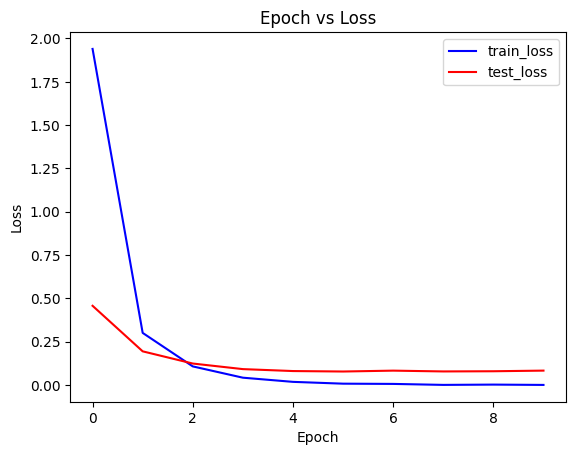
\includegraphics[width=1\textwidth]{./img/training-graph.png}
        \caption{Training graph}
    }
\end{figure}

